\documentclass{llncs}

\usepackage{graphicx}
\usepackage{mwe}
\usepackage{subfig}
\usepackage{amsmath}
\usepackage{amssymb}
\usepackage{rotating}

\begin{document}

\title{Numerical modelling of Lorenz system}
\author{Pawel Czyz}

\authorrunning{Pawel Czyz}

\institute{St Hugh's College, University of Oxford}

\maketitle

\begin{abstract}
We present a Python module implementing various ODE solvers, enabling one to do accurate and effective numerical simulations. We investigate it's accuracy investigating Lorenz chaotic system.

\keywords{numerical modelling, Runge-Kutta algorithm, chaos, Lorenz}
\end{abstract}

\section{Introduction}
In 1963 E. Lorenz modelling atmospheric convection proposed [1] a dynamical system:

\begin{align}
\label{eq:lorenz}
  y_0'&=a(y_1-y_0)\\
  y_1'&=ry_0-y_1-y_0y_2\\
  y_2'&=y_0y_1-by_2,
\end{align}

where $y_0$ is the rate of convection, $y_1$ and $y_2$ represent temperature changes in two dimensions and  $a,~b,~r$ are model constants related to Prandtl number, Rayleigh number and geometry of the convective layer.

As dynamical systems are in general hard problems to be solved analytically, Lorenz system is solved numerically. We decided to use classical Runge-Kutta method (RK4) [2, 3]. It allows one to integrate a dynamical
system:

\begin{equation}
  y'=f(y),
\end{equation}

where $y=(y_0, y_1,y_2)$ with a boundary condition $y(0)=(y_0^\circ, y_1^\circ, y_2^\circ)$.

Runge-Kutta method was implemented as a Python package allowing to track the whole history of the system as a function of time.

\section{Lorenz system}
We solved system (\ref{eq:lorenz}) for different ranges of parameter $r$ and obtained curve $y(t)$, which projections are shown in the Figure \ref{fig:yt}. While the system exhibits damped oscillations for $r\le 10$, starting at $r=28$, the system seems to behave chaotically\footnote{Proof that Lorenz system actually \textit{is} chaotic required huge computational power and can be found in [4].}.

A chaotic behaviour is also visible via temperature phase diagrams in the Figure \ref{fig:phase}. It makes simulations hugely dependent on initial boundary condition. In the Figure
\ref{fig:weather}. a time evolution of $y_0$ is presented for small perturbations in the boundary condition. Even for small (smaller than $1\%$) perturbations, the time evolution
becomes inaccurate after short period of time.

\begin{figure}
  \centering
  \begin{minipage}{.49\linewidth}
    \centering
    \subfloat[]{\label{fig:yt:a}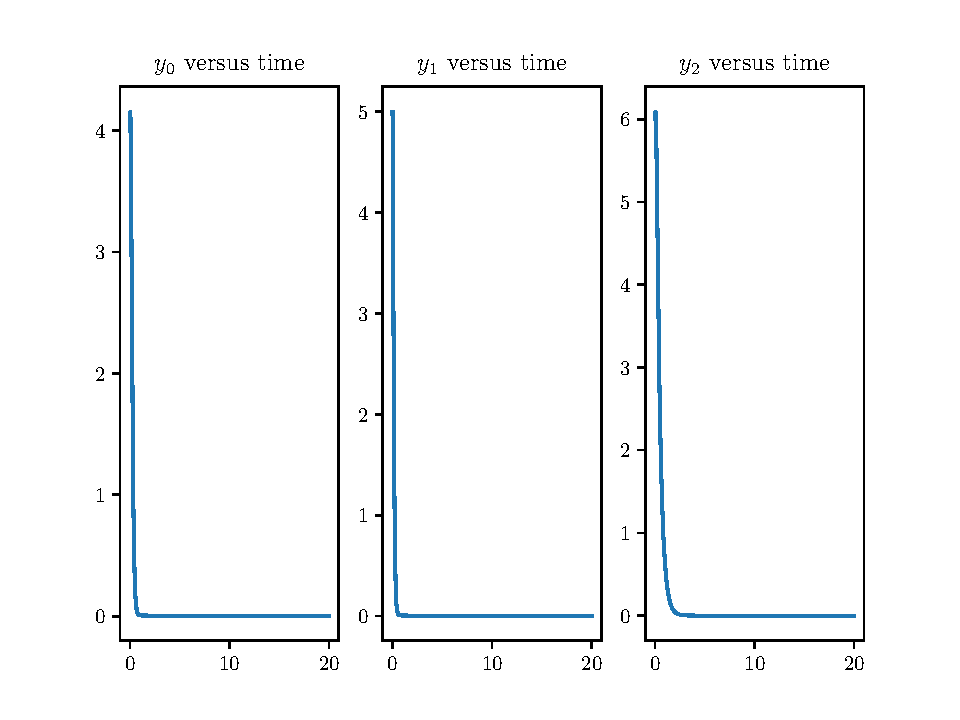
\includegraphics[width=\textwidth]{images/ys_vs_time-r_1}}
  \end{minipage}
  \begin{minipage}{.49\linewidth}
    \centering
    \subfloat[]{\label{fig:yt:b}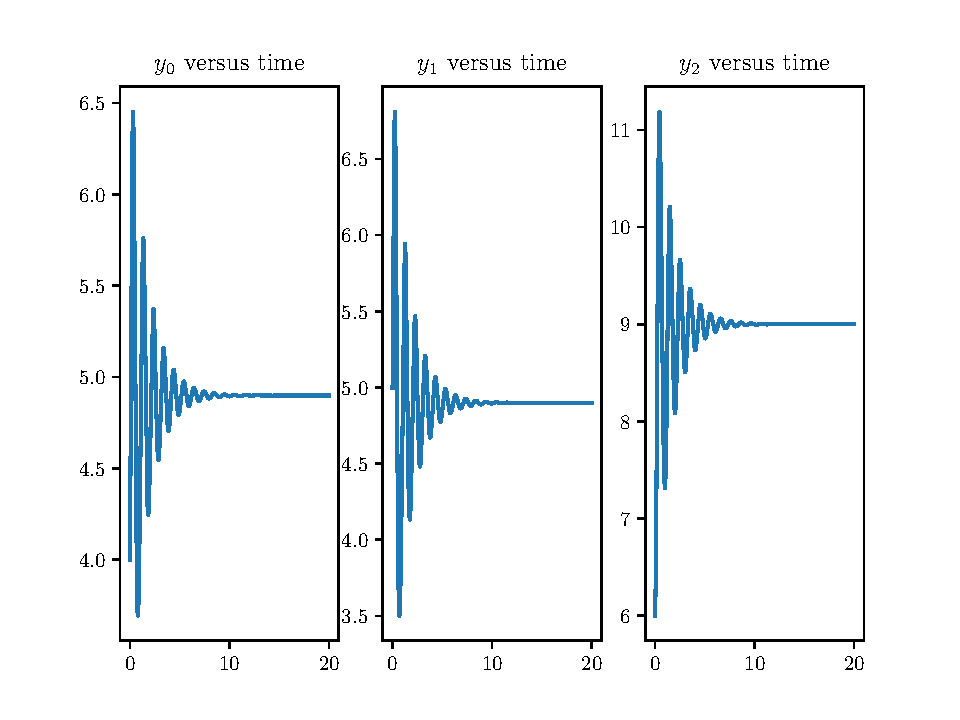
\includegraphics[width=\textwidth]{images/ys_vs_time-r_10}}
  \end{minipage}
  \\
  \begin{minipage}{.49\linewidth}
    \centering
    \subfloat[]{\label{fig:yt:c}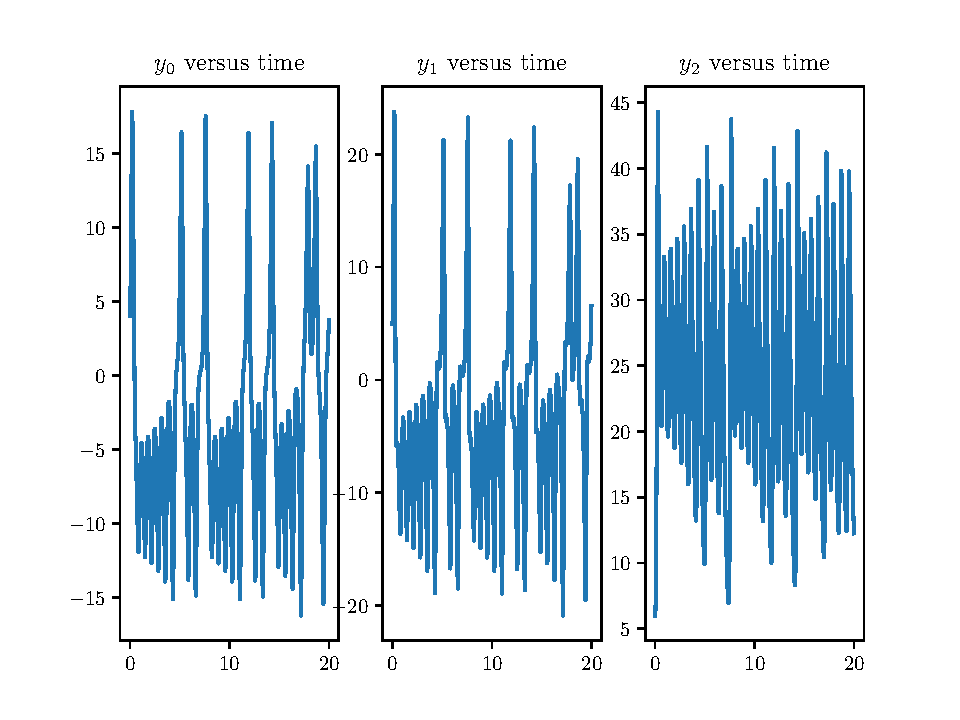
\includegraphics[width=\textwidth]{images/ys_vs_time-r_28}}
  \end{minipage}
  \begin{minipage}{.49\linewidth}
    \centering
    \subfloat[]{\label{fig:yt:d}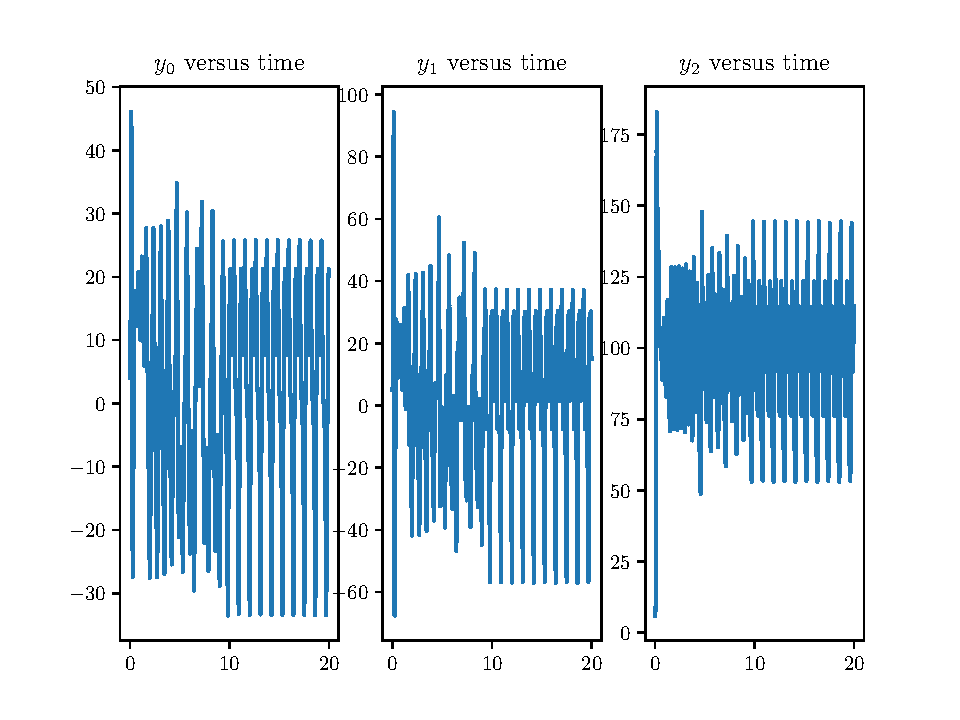
\includegraphics[width=\textwidth]{images/ys_vs_time-r_100}}
  \end{minipage}
  \caption{Solutions $y(t)$ for $y(0)=(4,5,6)$ and $a=10$, $b=8/3$. Model constant $r$ is different for every sub-figure:
  $r=1$ for \ref{fig:yt:a}, $r=10$ for \ref{fig:yt:b}, $r=28$ for \ref{fig:yt:c}. and $r=100$ for \ref{fig:yt:d}. We see a range of behaviours - for $r=1$ we see overdamped
  oscillations, for $r=10$ we see underdamped oscillations. Behaviour for $r=28$ and $r=100$ seems to be chaotic.}
\label{fig:yt}
\end{figure}

\begin{figure}
  \centering
  \begin{minipage}{.49\linewidth}
    \centering
    \subfloat[]{\label{fig:phase:a}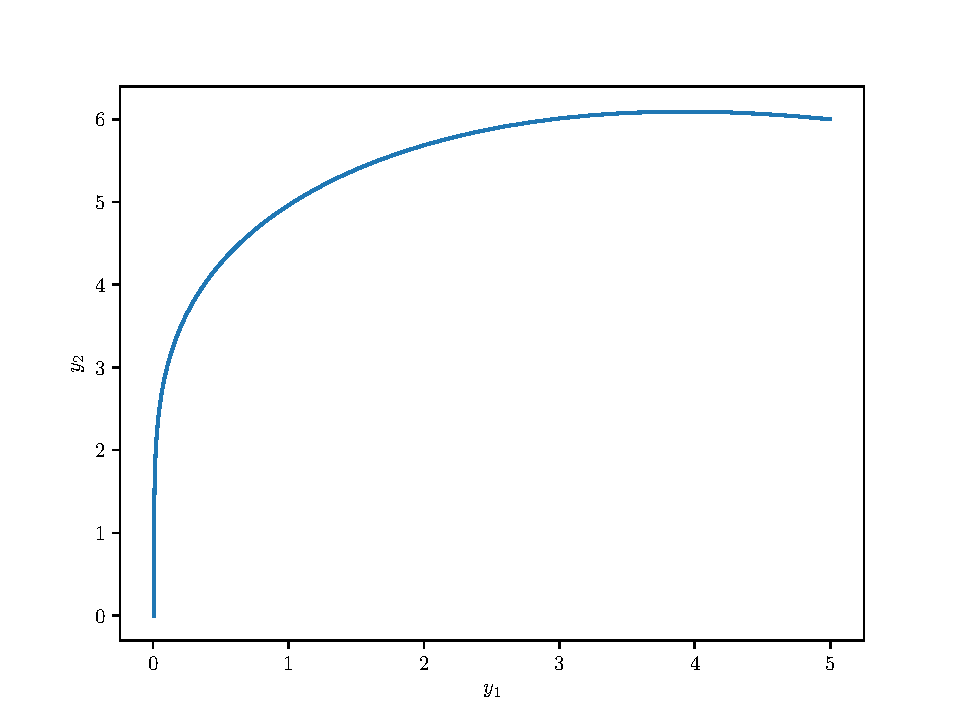
\includegraphics[width=\textwidth]{images/y1_vs_y2-r_1.pdf}}
  \end{minipage}
  \begin{minipage}{.49\linewidth}
    \centering
    \subfloat[]{\label{fig:phase:b}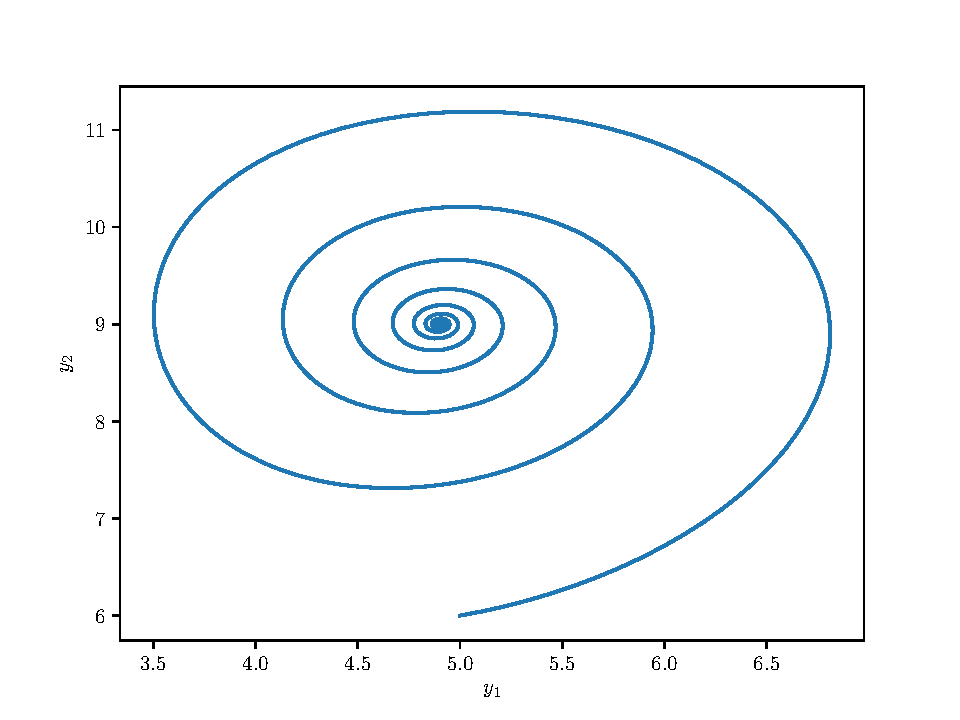
\includegraphics[width=\textwidth]{images/y1_vs_y2-r_10}}
  \end{minipage}
  \\
  \begin{minipage}{.49\linewidth}
    \centering
    \subfloat[]{\label{fig:phase:c}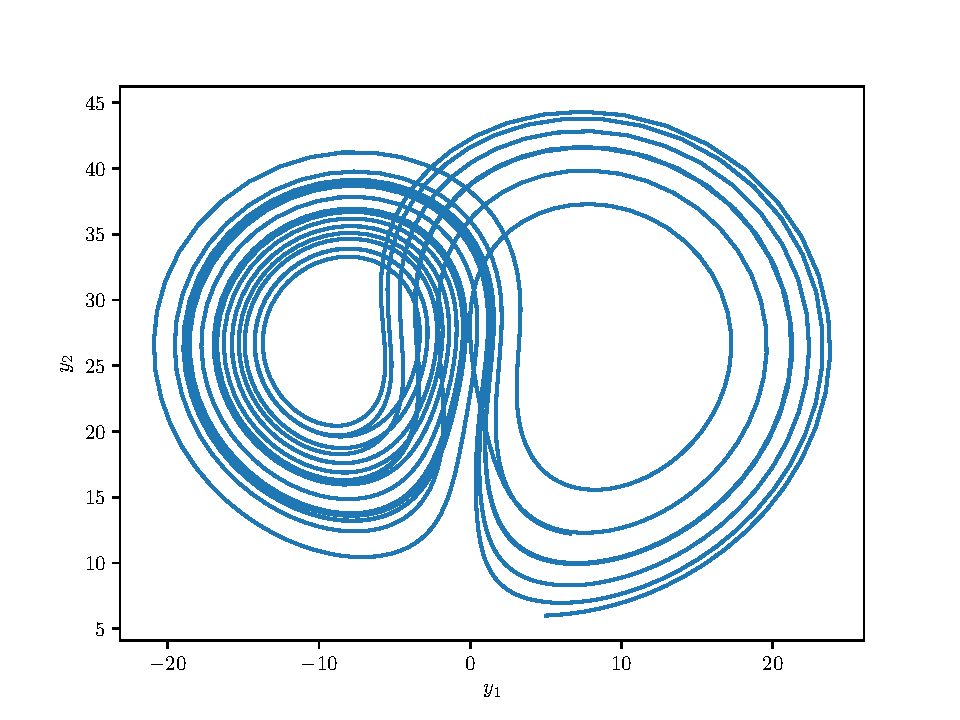
\includegraphics[width=\textwidth]{images/y1_vs_y2-r_28}}
  \end{minipage}
  \begin{minipage}{.49\linewidth}
    \centering
    \subfloat[]{\label{fig:phase:d}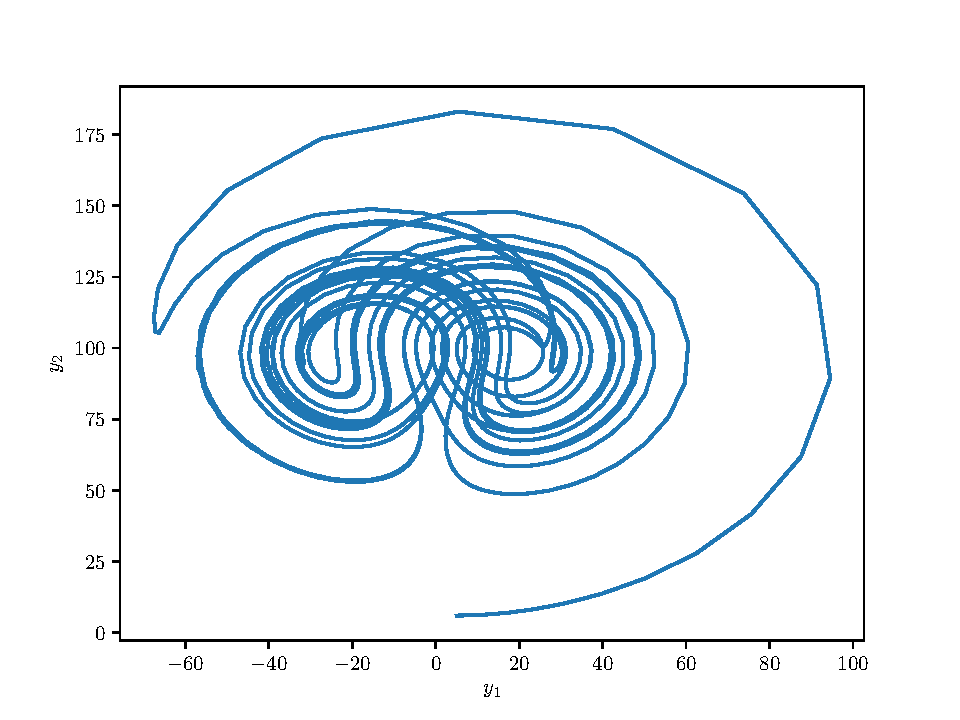
\includegraphics[width=\textwidth]{images/y1_vs_y2-r_100}}
  \end{minipage}
  \caption{Temperature phase diagrams (dependency between $y_1$ and $y_2$) for $y(0)=(4,5,6)$ and $a=10$, $b=8/3$. Model constant $r$ is different for every sub-figure:
  $r=1$ for \ref{fig:phase:a}, $r=10$ for \ref{fig:phase:b}, $r=28$ for \ref{fig:phase:c}. and $r=100$ for \ref{fig:phase:d}. We see a range of behaviours - for $r=1$ we see overdamped
  oscillations, for $r=10$ we see underdamped oscillations (a spiral is an ellipse, as in oscillation, with shrinking axes). Behaviour for $r=28$ and $r=100$ seems to be chaotic, butterfly-shaped Lorenz attractor is present.}
\label{fig:phase}
\end{figure}

\begin{figure}
  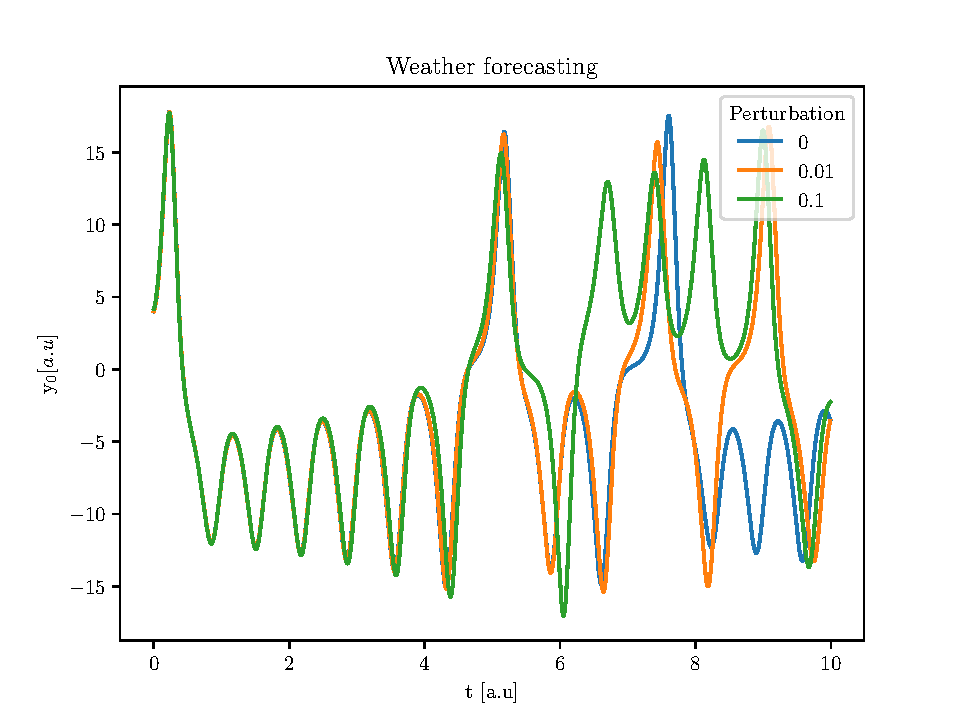
\includegraphics[width=\textwidth]{images/Weather_forecasting.pdf}
  \caption{Time evolution $y_0(t)$ for different boundary conditions. Model parameters are $a=10$, $b=8/3$, $r=28$. Boundary conditions vary as $y(0, p)=(4+p, 5+p, 6+p)$
  for $p$ taking values $0, 0.01, 0.1$. We see that after short period of time, perturbed curves become unrelated to the unperturbed curve.}
\label{fig:weather}
\end{figure}

\section{Conclusions}
We showed why weather forecasting is a hard problem by solving Lorenz system and investigating it's time evolution using own-implemented Runge-Kutta method. We showed that the system
can be believed to behave chaotically by investigation of phase diagrams and the dependency on perturbed initial conditions - smallest measurements errors in present increase exponentially with time. Created Python package can be also used to model different physical situations.

\section{References}
\begin{enumerate}
  \item E. Lorenz, Deterministic nonperiodic flow, Journal of the Atmospheric Sciences 20, 1963
  \item W. Press et al. Numerical Recipes: the Art of Scientific Computing, Cambridge University Press, 2007
  \item Joint work, Chaos Lab Script, University of Oxford, 2018
  \item B. Hassard et al. A Computer Proof that the Lorenz Equations Have “Chaotic” Solutions, Appl. Math. Lett. Vol. 7, 1994
\end{enumerate}

\end{document}
